\documentclass[10pt]{article}
\usepackage{fullpage}
\usepackage[utf8]{inputenc}
\usepackage{url}
\usepackage{graphicx}
%\renewcommand{\labelenumi}{(\alph{enumi})}
%\renewcommand{\labelenumii}{(\roman{enumii})}
\renewcommand{\labelenumi}{(\roman{enumi})}

\input macros

\begin{document}

\noindent TA: Ondřej Čertík\\
web: \url{http://hpfem.math.unr.edu/~ondrej/}\\
class: MATH 181\\
date: January 29, 2009

\section*{Quiz 4}

\subsection*{Problem 1}

Given a function $f(x)$:
$$f(x) = \cases{{x^2-x-6\over x-3}, &if $x\ne3$;\cr
                4, &if $x=3$.\cr}$$

\begin{enumerate}
\item Sketch the graph of the function
\item Is the function continuous at the point $x=3$? Why?
\end{enumerate}

\section*{Solution to Problem 1}

\begin{enumerate}
\item
We first rewrite the expression for $x\ne3$ into a simpler form, so that we can
sketch the graph:

$$f(x) = \cases{{x^2-x-6\over x-3}, &if $x\ne3$;\cr
                4, &if $x=3$.\cr}=
\cases{{(x-3)(x+2)\over x-3}, &if $x\ne3$;\cr
                4, &if $x=3$.\cr}=
\cases{{x+2}, &if $x\ne3$;\cr
                4, &if $x=3$.\cr}$$

Now we can sketch the graph:

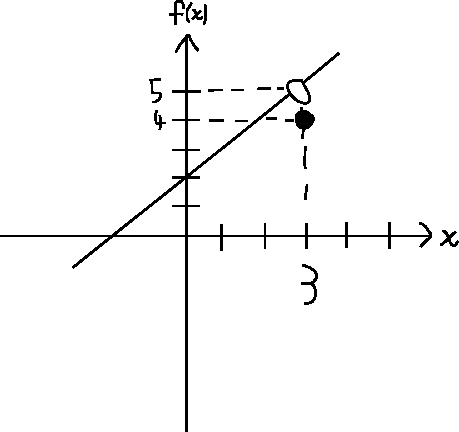
\includegraphics{diag1.pdf}

\item
The definition of a continuity at the point $x=3$ is:
$$\lim_{x\to3}f(x) = f(3)$$
If the equation holds, the function is continuous, if it doesn't, it is
discontinuous. In our case $f(3) = 4$ and
$$\lim_{x\to3}f(x) = \lim_{x\to3}x+2 = 5$$
so
$\lim_{x\to3}f(x) \ne f(3)$ and the function is not continuous at the point
$x=3$.


\end{enumerate}

\subsection*{Grading}

You got 4 points for rewriting:
$$f(x)=\cases{{x+2}, &if $x\ne3$;\cr
                4, &if $x=3$,\cr}$$
2 points for graphing the function and 4 points for correctly
determinning the continuity including the reasoning why.

\end{document}
